
%(BEGIN_QUESTION)
% Copyright 2010, Tony R. Kuphaldt, released under the Creative Commons Attribution License (v 1.0)
% This means you may do almost anything with this work of mine, so long as you give me proper credit

Suppose you are sent to troubleshoot a positive displacement flowmeter equipped with a pulse-contact output (rated at one pulse per 20 gallons), driving an electronic counter circuit to keep track of total water flow through the flowmeter over time.  The counter requires a {\it pulsing} signal to count up (i.e. a steady ``low'' or steady ``high'' signal will not result in an incrementing count value), and for some reason it is not counting as it should even though we know there is actually water flow going through the flowmeter.  Using a digital multimeter, you measure a constant 0 volts between terminals {\bf J} and {\bf K} while waiting long enough for the flowmeter switch to cycle (pulse) at least once:

$$\includegraphics[width=15.5cm]{i00372x01.eps}$$

Identify the likelihood of each specified fault for this circuit.  Consider each fault one at a time (i.e. no coincidental faults), determining whether or not each fault could independently account for {\it all} measurements and symptoms in this circuit.

% No blank lines allowed between lines of an \halign structure!
% I use comments (%) instead, so that TeX doesn't choke.

$$\vbox{\offinterlineskip
\halign{\strut
\vrule \quad\hfil # \ \hfil & 
\vrule \quad\hfil # \ \hfil & 
\vrule \quad\hfil # \ \hfil \vrule \cr
\noalign{\hrule}
%
% First row
{\bf Fault} & {\bf Possible} & {\bf Impossible} \cr
%
\noalign{\hrule}
%
% Another row
Flowmeter switch failed open &  &  \cr
%
\noalign{\hrule}
%
% Another row
Fuse blown (open) &  &  \cr
%
\noalign{\hrule}
%
% Another row
Open cable between C/D and E/F &  &  \cr
%
\noalign{\hrule}
%
% Another row
Resistor inside counter failed open &  &  \cr
%
\noalign{\hrule}
%
% Another row
Flowmeter switch failed shorted &  &  \cr
%
\noalign{\hrule}
%
% Another row
Shorted cable between C/D and E/F &  &  \cr
%
\noalign{\hrule}
%
% Another row
LED inside counter failed shorted &  &  \cr
%
\noalign{\hrule}
%
% Another row
Voltage source dead &  &  \cr
%
\noalign{\hrule}
} % End of \halign 
}$$ % End of \vbox

\underbar{file i00372}
%(END_QUESTION)





%(BEGIN_ANSWER)

% No blank lines allowed between lines of an \halign structure!
% I use comments (%) instead, so that TeX doesn't choke.

$$\vbox{\offinterlineskip
\halign{\strut
\vrule \quad\hfil # \ \hfil & 
\vrule \quad\hfil # \ \hfil & 
\vrule \quad\hfil # \ \hfil \vrule \cr
\noalign{\hrule}
%
% First row
{\bf Fault} & {\bf Possible} & {\bf Impossible} \cr
%
\noalign{\hrule}
%
% Another row
Flowmeter switch failed open & $\surd$ &  \cr
%
\noalign{\hrule}
%
% Another row
Fuse blown (open) & $\surd$ &  \cr
%
\noalign{\hrule}
%
% Another row
Open cable between C/D and E/F & $\surd$ &  \cr
%
\noalign{\hrule}
%
% Another row
Resistor inside counter failed open &  & $\surd$ \cr
%
\noalign{\hrule}
%
% Another row
Flowmeter switch failed shorted &  & $\surd$ \cr
%
\noalign{\hrule}
%
% Another row
Shorted cable between C/D and E/F &  & $\surd$ \cr
%
\noalign{\hrule}
%
% Another row
LED inside counter failed shorted &  & $\surd$ \cr
%
\noalign{\hrule}
%
% Another row
Voltage source dead & $\surd$ &  \cr
%
\noalign{\hrule}
} % End of \halign 
}$$ % End of \vbox


%(END_ANSWER)





%(BEGIN_NOTES)

{\bf This question is intended for exams only and not worksheets!}.

%(END_NOTES)

